% CRITERIA	(2-3 Pages)
	% -Stats & Distributions
% OUTLINE
	% - Distance of ours compared to the wavefront
	% - Dynamics, how often they are under an acceptable value
	% - How many times it finds a sucessful path w/o collisions
	% - Calculation time compared to wavefront
%
The following results were obtained through an experiment of 600 independent trials of the genetic algorithm in different environments. Robot configuration spaces were generated based on physical environments which featured objects randomly placed in the robot's path.

The number of test environment configurations was limited not by the genetically algorithm, but rather by the wavefront algorithm being used to validate results. Since the wavefront algorithm runtime approached 20 minutes per configuration, it was prohibitive to evaluate large numbers of possible environments in the available time.

Three configuration spaces were identified as good candidates for testing purposes, based on maps of varying complexity and obstacle density. Within each of these three environments, five sets of path start and end points were generated randomly. The points were checked to ensure that no invalid point configurations were present (i.e. conflicts situated within an obstacle). The algorithm was then run 40 times on each point set, and with five point sets per environment and three environments, a total of 600 trials were conducted.

Figure \ref{fig:res600} shows a visualization of 200 trials conducted on five start-end point sets on a populated configuration space. Note that each line in the visualization represents a full evolution cycle with a population of 75 individuals. While individual paths are obscured, the line densities show that the algorithm was able to determine a short and smooth trajectory in the majority of cases, with few outliers. The selected random point configurations exhibit both obscured and trivial problems (representative of a real-world environment). The results of the experiment are presented in Table \ref{tbl:results}.

\begin{figure}[h]
	\centering
	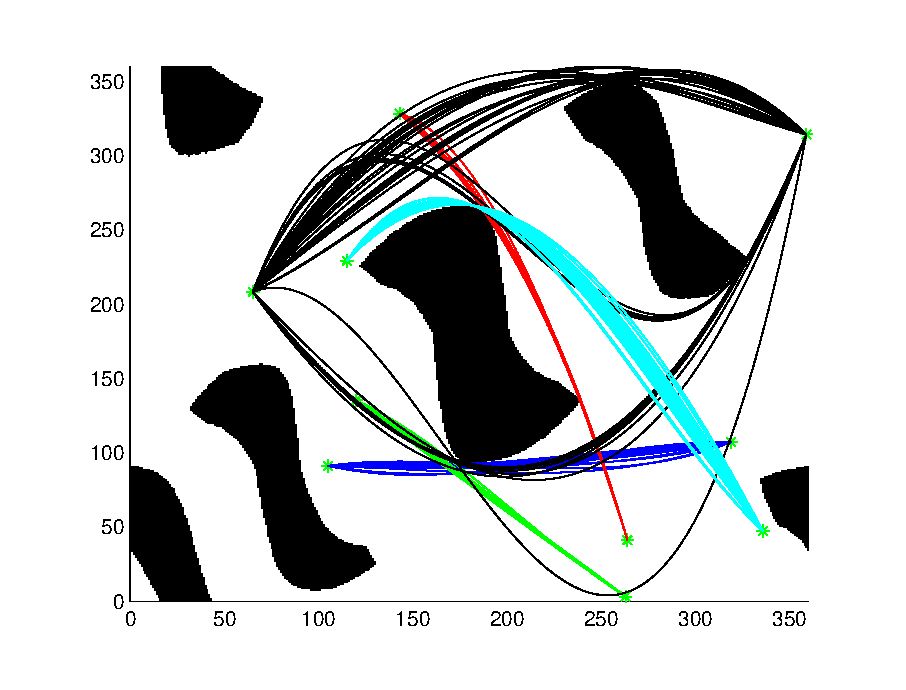
\includegraphics[width=\figWidth]{./figures/results_cSpace4.eps}
	\caption{Resulting paths from 200 independent trials, between five start-end point configurations in a single environment. Each path is the result of a full life-cycle of the algorithm. Paths show the algorithm consistently identifies the shortest path, with few outliers.}
	\label{fig:res600}
\end{figure}

\begin{table}
\renewcommand{\arraystretch}{1.4}
\caption{Agregated results of 600 trials of the path finding algorithm, between 15 environment configurations.}
\label{tbl:results}
\begin{center}
		\begin{tabular}{ c | c  c  p{1.8cm} }
		Criteria & Result & Unit & Note \\ \hline
		Path length & 0.7 & \% longer & Compared to wavefront method \\
		Freq. of shorter path & 79 & \% & Compared to wavefront method \\
		Time to completion & 5.15 & seconds & 20767\% improvement on wavefront method \\
		Average number of generations & 12.3 & generations & \\
		Freq. of collision-free path & 94 & \% &  \\
		Jerk improvement & 194 & ${\frac{D}{T^3}}$ & Compared to implementation not minimizing jerk.\\
\end{tabular}
\end{center}
\end{table}